% Options for packages loaded elsewhere
\PassOptionsToPackage{unicode}{hyperref}
\PassOptionsToPackage{hyphens}{url}
\PassOptionsToPackage{dvipsnames,svgnames,x11names}{xcolor}
%
\documentclass[
  12pt,
  oneside,
  a4paper,
  chapter=TITLE,
  section=TITLE,
  brazil]{abntex2}

\usepackage{amsmath,amssymb}
\usepackage{lmodern}
\usepackage{iftex}
\ifPDFTeX
  \usepackage[T1]{fontenc}
  \usepackage[utf8]{inputenc}
  \usepackage{textcomp} % provide euro and other symbols
\else % if luatex or xetex
  \usepackage{unicode-math}
  \defaultfontfeatures{Scale=MatchLowercase}
  \defaultfontfeatures[\rmfamily]{Ligatures=TeX,Scale=1}
\fi
% Use upquote if available, for straight quotes in verbatim environments
\IfFileExists{upquote.sty}{\usepackage{upquote}}{}
\IfFileExists{microtype.sty}{% use microtype if available
  \usepackage[]{microtype}
  \UseMicrotypeSet[protrusion]{basicmath} % disable protrusion for tt fonts
}{}
\makeatletter
\@ifundefined{KOMAClassName}{% if non-KOMA class
  \IfFileExists{parskip.sty}{%
    \usepackage{parskip}
  }{% else
    \setlength{\parindent}{0pt}
    \setlength{\parskip}{6pt plus 2pt minus 1pt}}
}{% if KOMA class
  \KOMAoptions{parskip=half}}
\makeatother
\usepackage{xcolor}
\setlength{\emergencystretch}{3em} % prevent overfull lines
\setcounter{secnumdepth}{5}
% Make \paragraph and \subparagraph free-standing
\ifx\paragraph\undefined\else
  \let\oldparagraph\paragraph
  \renewcommand{\paragraph}[1]{\oldparagraph{#1}\mbox{}}
\fi
\ifx\subparagraph\undefined\else
  \let\oldsubparagraph\subparagraph
  \renewcommand{\subparagraph}[1]{\oldsubparagraph{#1}\mbox{}}
\fi


\providecommand{\tightlist}{%
  \setlength{\itemsep}{0pt}\setlength{\parskip}{0pt}}\usepackage{longtable,booktabs,array}
\usepackage{calc} % for calculating minipage widths
% Correct order of tables after \paragraph or \subparagraph
\usepackage{etoolbox}
\makeatletter
\patchcmd\longtable{\par}{\if@noskipsec\mbox{}\fi\par}{}{}
\makeatother
% Allow footnotes in longtable head/foot
\IfFileExists{footnotehyper.sty}{\usepackage{footnotehyper}}{\usepackage{footnote}}
\makesavenoteenv{longtable}
\usepackage{graphicx}
\makeatletter
\def\maxwidth{\ifdim\Gin@nat@width>\linewidth\linewidth\else\Gin@nat@width\fi}
\def\maxheight{\ifdim\Gin@nat@height>\textheight\textheight\else\Gin@nat@height\fi}
\makeatother
% Scale images if necessary, so that they will not overflow the page
% margins by default, and it is still possible to overwrite the defaults
% using explicit options in \includegraphics[width, height, ...]{}
\setkeys{Gin}{width=\maxwidth,height=\maxheight,keepaspectratio}
% Set default figure placement to htbp
\makeatletter
\def\fps@figure{htbp}
\makeatother

% opções para o classoption
%
%	12pt,				% tamanho da fonte
%	openright,			% capítulos começam em pág ímpar (insere página vazia caso preciso)
%	twoside,			% para impressão em recto e verso. Oposto a oneside
%	a4paper,			% tamanho do papel. 
%	% -- opções da classe abntex2 --
%	%chapter=TITLE,		% títulos de capítulos convertidos em letras maiúsculas
%	%section=TITLE,		% títulos de seções convertidos em letras maiúsculas
%	%subsection=TITLE,	% títulos de subseções convertidos em letras maiúsculas
%	%subsubsection=TITLE,% títulos de subsubseções convertidos em letras maiúsculas
%	% -- opções do pacote babel --
%	english,			% idioma adicional para hifenização
%	french,				% idioma adicional para hifenização
%	spanish,			% idioma adicional para hifenização
%	brazil				% o último idioma é o principal do documento

% ---
% Pacotes básicos 
% ---
\usepackage{lmodern}			% Usa a fonte Latin Modern			
\usepackage[T1]{fontenc}		% Selecao de codigos de fonte.
\usepackage[utf8]{inputenc}		% Codificacao do documento (conversão automática dos acentos)
\usepackage{indentfirst}		% Indenta o primeiro parágrafo de cada seção.
\usepackage{color}				% Controle das cores
\usepackage{graphicx}			% Inclusão de gráficos
\usepackage{microtype} 			% para melhorias de justificação
\usepackage{config/ppgecotex}	% customização para PPGEco/UFES
% ---

% ---
% Pacotes adicionais
% ---
\usepackage{lipsum}																% para geração de dummy text
\usepackage{bbm, times, quoting, setspace, lscape}
\usepackage{psfrag, fancyhdr}
\usepackage{amsmath, amsfonts, amssymb, amsthm}									% escrita matemática
\usepackage{xcolor, url, placeins, enumitem}
\usepackage{dcolumn, lastpage}
\usepackage[skip = 2pt, size = normalsize, labelfont = bf]{caption}
% ---

% ---
% Pacotes de citações
% ---
\usepackage[backend=biber, style=abnt, ittitles, justify, indent, backref=true]{biblatex}

% fontes
\setmainfont{Times New Roman}
\setmonofont[Scale=0.9, Scale=MatchLowercase]{Consolas}

% --- 
% CONFIGURAÇÕES DE PACOTES
% --- 

% ---
% Configurações de aparência do PDF final

% alterando o aspecto da cor azul
\definecolor{blue}{RGB}{41,5,195}

% informações do PDF
\makeatletter
\hypersetup{
     	%pagebackref=true,
		pdftitle={\@title}, 
		pdfauthor={\@author},
    	pdfsubject={\imprimirpreambulo},
	    pdfcreator={LaTeX with abnTeX2},
		pdfkeywords={abnt}{latex}{abntex}{abntex2}{trabalho acadêmico}, 
		colorlinks=true,       		% false: boxed links; true: colored links
    	linkcolor=blue,          	% color of internal links
    	citecolor=blue,        		% color of links to bibliography
    	filecolor=magenta,      		% color of file links
		urlcolor=blue,
		bookmarksdepth=4
}
\makeatother
% --- 

% ---
% Posiciona figuras e tabelas no topo da página quando adicionadas sozinhas
% em um página em branco. Ver https://github.com/abntex/abntex2/issues/170
\makeatletter
\setlength{\@fptop}{5pt} % Set distance from top of page to first float
\makeatother
% ---

% ---
% Possibilita criação de Quadros e Lista de quadros.
% Ver https://github.com/abntex/abntex2/issues/176
%
\newcommand{\quadroname}{Quadro}
\newcommand{\listofquadrosname}{Lista de Quadros}

\newfloat[chapter]{quadro}{loq}{\quadroname}
\newlistof{listofquadros}{loq}{\listofquadrosname}
\newlistentry{quadro}{loq}{0}

% configurações para atender às regras da ABNT
\setfloatadjustment{quadro}{\centering}
\counterwithout{quadro}{chapter}
\renewcommand{\cftquadroname}{\quadroname\space} 
\renewcommand*{\cftquadroaftersnum}{\hfill--\hfill}

\setfloatlocations{quadro}{hbtp} % Ver https://github.com/abntex/abntex2/issues/176
% ---

% --- 
% Espaçamentos entre linhas e parágrafos 
% --- 

% O tamanho do parágrafo é dado por:
\setlength{\parindent}{1.3cm}

% Controle do espaçamento entre um parágrafo e outro:
\setlength{\parskip}{0.2cm}  % tente também \onelineskip

% ---
% compila o indice
% ---
\makeindex
% ---

% Seleciona o idioma do documento (conforme pacotes do babel)
%\selectlanguage{english}
\selectlanguage{brazil}
\captionsetup[figure]{name=Figura}
\captionsetup[table]{name=Tabela}

% Retira espaço extra obsoleto entre as frases.
\frenchspacing 

% matrizes
\setcounter{MaxMatrixCols}{20}

% bibliografia
\addbibresource{config/Dissertação.bib}
\addbibresource{config/packages.bib}

% fazer sumário começar do 1 ao invés do zero
\renewcommand{\thesection}{\arabic{section}}

% posição das figuras
\setfloatlocations{figure}{hbtp}
\setfloatlocations{table}{hbtp}
\titulo{MÉTODOS DE MACHINE LEARNING PARA RECONCILIAÇÃO ÓTIMA DE SÉRIES TEMPORAIS HIERÁRQUICAS E AGRUPADAS}
\local{VITÓRIA}
\orientador{Prof. Dr. Guilherme A. A. Pereira}
\instituicao{%
    UNIVERSIDADE FEDERAL DO ESPÍRITO SANTO
    \par
    CENTRO DE CIÊNCIAS JURÍDICAS E ECONÔMICAS
    \par
    PROGRAMA DE PÓS-GRADUAÇÃO EM ECONOMIA}
\tipotrabalho{Dissertação (Mestrado)}
\preambulo{Dissertação apresentada ao Programa de Pós-Graduação em Economia da Universidade Federal do Espírito Santo, como requisito para a obtenção do título de Mestre em Economia.}
\usepackage{booktabs}
\usepackage{longtable}
\usepackage{array}
\usepackage{multirow}
\usepackage{wrapfig}
\usepackage{float}
\usepackage{colortbl}
\usepackage{pdflscape}
\usepackage{tabu}
\usepackage{threeparttable}
\usepackage{threeparttablex}
\usepackage[normalem]{ulem}
\usepackage{makecell}
\usepackage{xcolor}
\makeatletter
\makeatother
\makeatletter
\makeatother
\makeatletter
\@ifpackageloaded{caption}{}{\usepackage{caption}}
\AtBeginDocument{%
\ifdefined\contentsname
  \renewcommand*\contentsname{Table of contents}
\else
  \newcommand\contentsname{Table of contents}
\fi
\ifdefined\listfigurename
  \renewcommand*\listfigurename{LISTA DE FIGURAS}
\else
  \newcommand\listfigurename{LISTA DE FIGURAS}
\fi
\ifdefined\listtablename
  \renewcommand*\listtablename{LISTA DE TABELAS}
\else
  \newcommand\listtablename{LISTA DE TABELAS}
\fi
\ifdefined\figurename
  \renewcommand*\figurename{Figure}
\else
  \newcommand\figurename{Figure}
\fi
\ifdefined\tablename
  \renewcommand*\tablename{Table}
\else
  \newcommand\tablename{Table}
\fi
}
\@ifpackageloaded{float}{}{\usepackage{float}}
\floatstyle{ruled}
\@ifundefined{c@chapter}{\newfloat{codelisting}{h}{lop}}{\newfloat{codelisting}{h}{lop}[chapter]}
\floatname{codelisting}{Listing}
\newcommand*\listoflistings{\listof{codelisting}{List of Listings}}
\makeatother
\makeatletter
\@ifpackageloaded{caption}{}{\usepackage{caption}}
\@ifpackageloaded{subcaption}{}{\usepackage{subcaption}}
\makeatother
\makeatletter
\@ifpackageloaded{tcolorbox}{}{\usepackage[many]{tcolorbox}}
\makeatother
\makeatletter
\@ifundefined{shadecolor}{\definecolor{shadecolor}{rgb}{.97, .97, .97}}
\makeatother
\makeatletter
\makeatother
\ifLuaTeX
  \usepackage{selnolig}  % disable illegal ligatures
\fi
\usepackage[]{biblatex}
\IfFileExists{bookmark.sty}{\usepackage{bookmark}}{\usepackage{hyperref}}
\IfFileExists{xurl.sty}{\usepackage{xurl}}{} % add URL line breaks if available
\urlstyle{same} % disable monospaced font for URLs
\hypersetup{
  pdfauthor={ALBERSON DA SILVA MIRANDA},
  colorlinks=true,
  linkcolor={blue},
  filecolor={Maroon},
  citecolor={Blue},
  urlcolor={Blue},
  pdfcreator={LaTeX via pandoc}}

\author{ALBERSON DA SILVA MIRANDA}
\date{2023}

\begin{document}
% elementos pré-textuais 

% título do sumário
\ifdefined\contentsname
  \renewcommand*\contentsname{SUMÁRIO}
\else
  \newcommand\contentsname{SUMÁRIO}
\fi

% capa 
\imprimircapa

% folha de rosto 
% o * indica que haverá a ficha bibliográfica 
\imprimirfolhaderosto*

% ficha catalográfica 
%\begin{fichacatalografica}
%    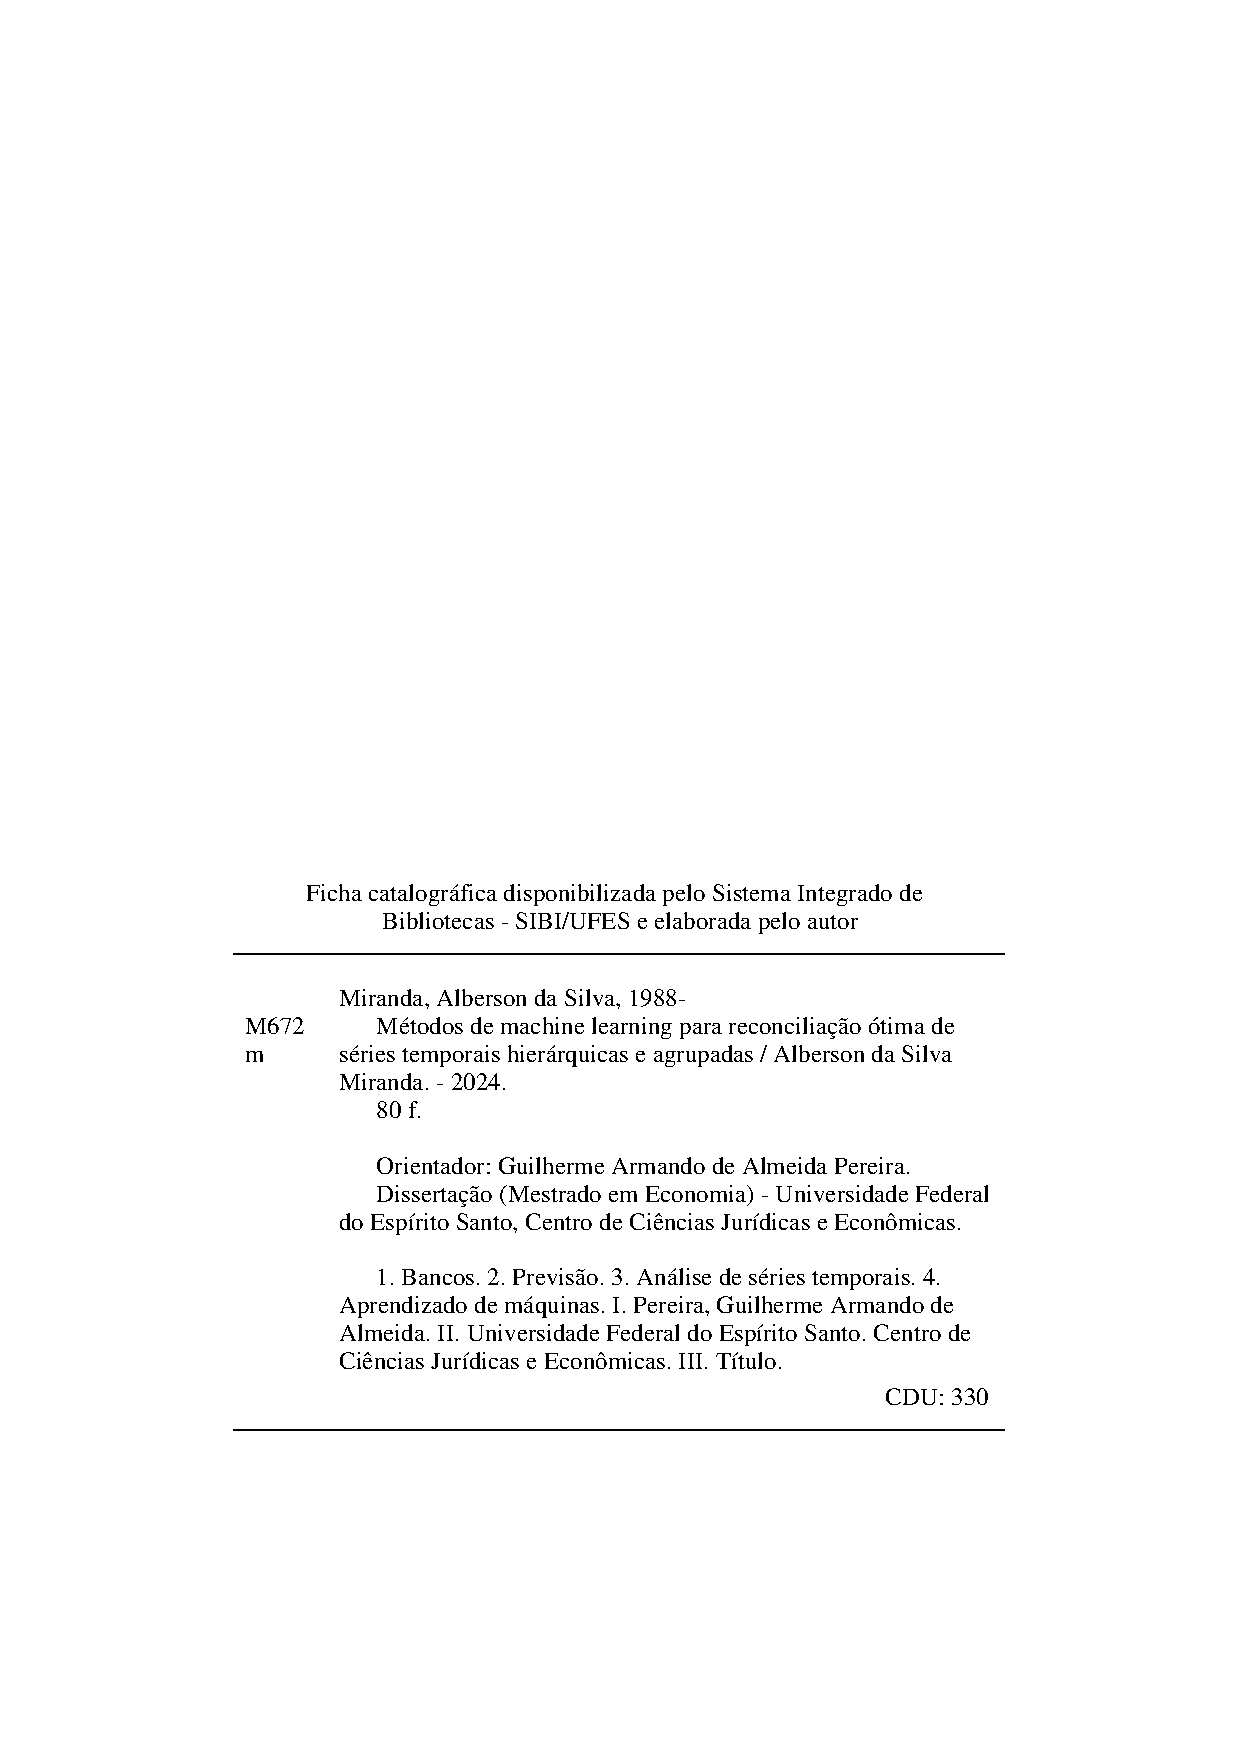
\includepdf{ficha_ufes.pdf}
%\end{fichacatalografica}


% substituir pela ficha em pdf fornecida pela UFES após defesa 
\begin{fichacatalografica}
	\sffamily
	\vspace*{\fill}					% Posição vertical
	\begin{center}					% Minipage Centralizado
	\fbox{\begin{minipage}[c][8cm]{15cm}		% Largura
	\small
	\imprimirautor
	
	\hspace{0.5cm} \imprimirtitulo  / \imprimirautor. --
	\imprimirlocal, \imprimirdata-
	
	\hspace{0.5cm} \thelastpage p. : il. (algumas color.) ; 30 cm.\\
	
	\hspace{0.5cm} \imprimirorientadorRotulo~\imprimirorientador\\
	
	\hspace{0.5cm}
	\parbox[t]{\textwidth}{\imprimirtipotrabalho~--~\imprimirinstituicao,
	\imprimirdata.}\\
	
	\hspace{0.5cm}
		1. Palavra-chave1.
		2. Palavra-chave2.
		2. Palavra-chave3.
		I. Orientador.
		II. Universidade xxx.
		III. Faculdade de xxx.
		IV. Título 			
	\end{minipage}}
	\end{center}
\end{fichacatalografica}

% folha de aprovação 
%
%\begin{folhadeaprovacao}
%    \includepdf{folhadeaprovacao_final.pdf}
%\end{folhadeaprovacao}


% substituir pela folha assinada pela banca após defesa 
\begin{folhadeaprovacao}

  \begin{center}
    {\ABNTEXchapterfont\large\imprimirautor}

    \vspace*{\fill}\vspace*{\fill}
    \begin{center}
      \ABNTEXchapterfont\bfseries\Large\imprimirtitulo
    \end{center}
    \vspace*{\fill}
    
    \hspace{.45\textwidth}
    \begin{minipage}{.5\textwidth}
        \imprimirpreambulo
        \vspace*{1cm}
        Aprovada em xx de xx de 20xx.\\[2cm]
        \textbf{COMISSÃO EXAMINADORA} \\
        \assinatura{\textbf{\imprimirorientador} \\ Universidade Federal do Espírito Santo \\ Orientador} 
        \assinatura{\textbf{Professor} \\ Instituição}
        \assinatura{\textbf{Professor} \\ Instituição}
        %\assinatura{\textbf{Professor} \\ Convidado 3}
        %\assinatura{\textbf{Professor} \\ Convidado 4}
    \end{minipage}%
   \end{center}
  
\end{folhadeaprovacao}

%% dedicatória 
%\begin{dedicatoria}
%   \vspace*{\fill}
%   \centering
%   \noindent
%   \textit{Exemplo de dedicatória,\\\lipsum[10].} \vspace*{\fill}
%\end{dedicatoria}

%% agradecimentos 
%\begin{agradecimentos}
%\lipsum[30]
%
%\lipsum[30]
%
%\end{agradecimentos}

% epígrafe 
%\begin{epigrafe}
%    \vspace*{\fill}
%	\begin{flushright}
%		\textit{``Modelo de epígrafe, \\
%		modelo de epígrafe.''}
%	\end{flushright}
%\end{epigrafe}

% resumo 

\setlength{\absparsep}{18pt}
\begin{resumo}
  \lipsum[30]

  \textbf{Palavras-chave}: palavra-chave1. palavra-chave2. palavra-chave3.
\end{resumo}

% abstract 
\begin{resumo}[Abstract]
  \begin{otherlanguage*}{english}
    \lipsum[30]

    \vspace{\onelineskip}
 
    \noindent 
    \textbf{Keywords}: keyword1. keyword2. keyword3.
  \end{otherlanguage*}
\end{resumo}

% lista de ilustrações 
\pdfbookmark[0]{\listfigurename}{lof}
\listoffigures*
\cleardoublepage

% lista de quadros 
\pdfbookmark[0]{\listofquadrosname}{loq}
\listofquadros*
\cleardoublepage

% lista de tabelas 
\pdfbookmark[0]{\listtablename}{lot}
\listoftables*
\cleardoublepage

% lista de abreviaturas 
\begin{siglas}
  \item[MinT] \textit{Minimum Trace}
  \item[MCRL] Modelo Clássico de Regressão Linear
  \item[MQO] Mínimos Quadrados Ordinários
  \item[MQP] Mínimos Quadrados Ponderados
\end{siglas}

% lista de símbolos 
\begin{simbolos}
  \item[$ t $] Tempo dentro da amostra
  \item[$ T $] Último tempo dentro da amostra, quantidade de observações numa série
  \item[$ h $] Horizonte de previsão, tempo fora da amostra
  \item[$ \Omega $] Conjunto de dados dentro da amostra
  \item[$ y $] Série temporal dentro da amostra
  \item[$ \hat{y} $] Série temporal estimada
  \item[$ \tilde{y} $] Série temporal reconciliada
  \item[$ n $] Número de séries na hierarquia
  \item[$ m $] Número de séries no menor nível da hierarquia
  \item[$ k $] Número de níveis na hierarquia
  \item[$ \mathbfit{S} $] Matriz de soma
  \item[$ \mathbfit{G} $] Matriz de reconciliação
  \item[$\{...\}$] Conjunto
  \item[$|\{...\}|$] Número de elementos em um conjunto
\end{simbolos}

% sumário 
\pdfbookmark[0]{\contentsname}{toc}
\tableofcontents*
\cleardoublepage

% elementos textuais 
\textual

\ifdefined\Shaded\renewenvironment{Shaded}{\begin{tcolorbox}[boxrule=0pt, breakable, interior hidden, enhanced, frame hidden, borderline west={3pt}{0pt}{shadecolor}, sharp corners]}{\end{tcolorbox}}\fi

\hypertarget{introduuxe7uxe3o}{%
\section{INTRODUÇÃO}\label{introduuxe7uxe3o}}

Neste trabalho,

\hypertarget{suxe9ries-hieruxe1rquicas-e-suxe9ries-agrupadas}{%
\subsection{Séries hierárquicas e séries
agrupadas}\label{suxe9ries-hieruxe1rquicas-e-suxe9ries-agrupadas}}

Séries temporais hierárquicas são aquelas que podem ser agregadas ou
desagregadas naturalmente em uma estrutura aninhada
\autocite{hyndman_forecasting_2021}. Para ilustrar, tome a série do PIB
brasileiro. Ela pode ser desagregada por estado que, por sua vez, pode
ser desagregada por município.

\begin{figure}

{\centering 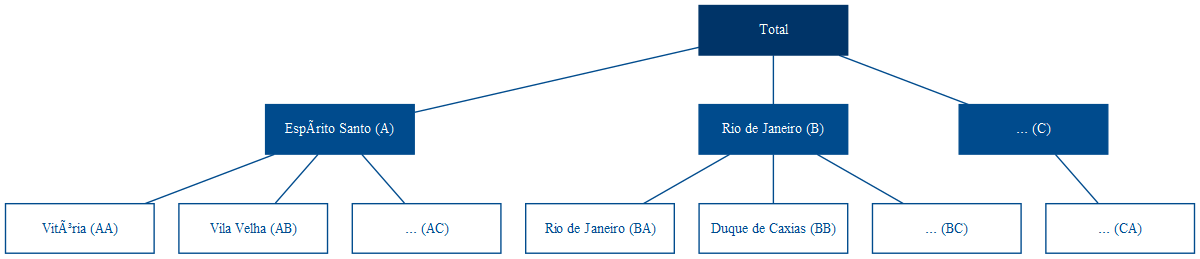
\includegraphics{img/hierarq.png}

}

\caption{\label{fig-h}Séries Hierárquicas}

\end{figure}

Essa estrutura pode ser representada por equações para qualquer nível de
agregação.

\begin{align}
y_t &= y_{A,t} + y_{B,t} + y_{C,t} \label{eq:ha} \\
y_t &= y_{AA,t} + y_{AB,t} + y_{AC,t} + y_{BA,t} + y_{BC,t} + y_{CA,t}\label{eq:ha_mun} \\
y_{A,t} &= y_{AA,t} + y_{AB,t} + y_{AC,t} \label{eq:haES}
\end{align}

Assim, o agregado nacional pode ser representado apenas pelos agregados
dos estados, através de \eqref{eq:ha}, ou como o agregado dos municípios
\eqref{eq:ha_mun}. Já o agregado para o estado do Espírito Santo é
representado por \eqref{eq:haES}.

Alternativamente, podemos descrever a estrutura completa de forma
matricial:

\begin{equation}\protect\hypertarget{eq-matriz_hierarquia}{}{
\begin{bmatrix}
    y_{t} \\
    y_{A, t} \\
    y_{B, t} \\
    y_{C, t} \\
    y_{AA, t} \\
    y_{AB, t} \\
    y_{AC, t} \\
    y_{BA, t} \\
    y_{BB, t} \\
    y_{BC, t} \\
    y_{CA, t}
\end{bmatrix}
=
\begin{bmatrix}
    1 & 1 & 1 & 1 & 1 & 1 & 1 \\
    1 & 1 & 1 & 0 & 0 & 0 & 0 \\
    0 & 0 & 0 & 1 & 1 & 1 & 0 \\
    0 & 0 & 0 & 0 & 0 & 0 & 1 \\
    1 & 0 & 0 & 0 & 0 & 0 & 0 \\
    0 & 1 & 0 & 0 & 0 & 0 & 0 \\
    0 & 0 & 1 & 0 & 0 & 0 & 0 \\
    0 & 0 & 0 & 1 & 0 & 0 & 0 \\
    0 & 0 & 0 & 0 & 1 & 0 & 0 \\
    0 & 0 & 0 & 0 & 0 & 1 & 0 \\
    0 & 0 & 0 & 0 & 0 & 0 & 1 \\
\end{bmatrix}
\begin{bmatrix}
    y_{AA, t} \\
    y_{AB, t} \\
    y_{AC, t} \\
    y_{BA, t} \\
    y_{BB, t} \\
    y_{BC, t} \\
    y_{CA, t}
\end{bmatrix}
}\label{eq-matriz_hierarquia}\end{equation}

Por outro lado, o PIB pode ser também desagregado de forma cruzada de
acordo com a atividade econômica --- lavoura, rebanho, indústria de
transformação, extrativa, bens de capital, bens intermediários, comércio
de vestuário, automotivos, serviços etc. Essa estrutura não pode ser
desagregada naturalmente de uma única forma, como é a hierarquia de
estados e municípios. Não pode ser aninhada por um atributo como a
própria geografia. A esse tipo de estrutura dá-se o nome de séries
agrupadas.

\begin{figure}

{\centering 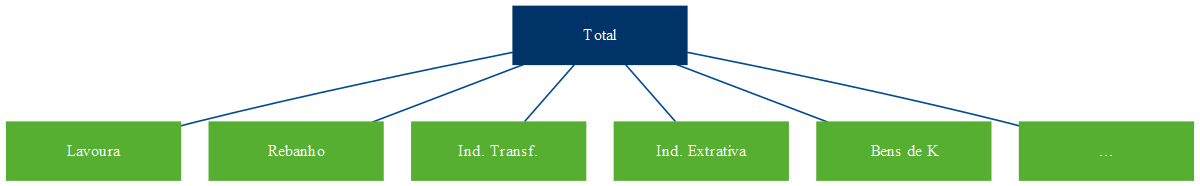
\includegraphics{img/agrupadas.png}

}

\caption{\label{fig-a}Séries Agrupadas}

\end{figure}

Combinando as duas, temos a estrutura de séries hierárquicas agrupadas.
Ao contrário da estrutura hierárquica, que só pode ser agregada de uma
forma --- como com os municípios abaixo dos estados ---, a adição da
estrutura agrupada pode ocorrer tanto acima (Figura~\ref{fig-ha1})
quanto abaixo (Figura~\ref{fig-ha2}) da hierárquica.

\begin{figure}

{\centering 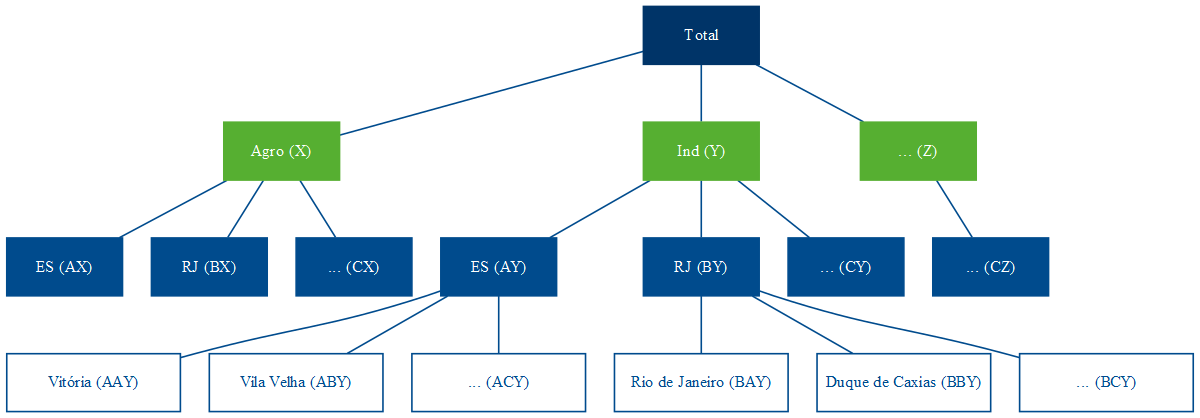
\includegraphics{img/hier_agrup.png}

}

\caption{\label{fig-ha1}Séries Hierárquicas Agrupadas (a)}

\end{figure}

\begin{figure}

{\centering 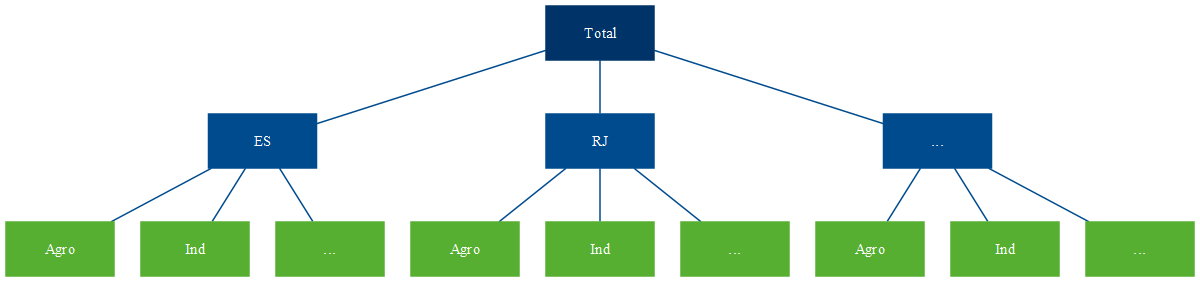
\includegraphics{img/hier_agrup_2.png}

}

\caption{\label{fig-ha2}Séries Hierárquicas Agrupadas (b)}

\end{figure}

Na notação matricial, a estrutura da Figura~\ref{fig-ha2} é representada
como abaixo. Formalmente, o primeiro membro da igualdade é composto pelo
vetor \(\mathbfit{y}_t\) \(n\)-dimensional com todas as observações no
tempo \(t\) para todos os níveis da hierarquia. O segundo membro é
composto pela matriz de soma \(\mathbfit{S}\) \index{matriz de soma}de
dimensão \(n \times m\) que define as equações para todo nível de
agregação, e pela matriz \(\mathbfit{b}_t\) composta pelas séries no
nível mais desagregado.

\[
\mathbfit{y}_t=\mathbfit{Sb}_t
\]

\begin{equation}\protect\hypertarget{eq-matriz_ha}{}{
\begin{bmatrix}
    y_{t} \\
    y_{A, t} \\
    y_{B, t} \\
    y_{C, t} \\
    y_{X, t} \\
    y_{Y, t} \\
    y_{Z, t} \\
    y_{AX, t} \\
    y_{AY, t} \\
    y_{AZ, t} \\
    y_{BX, t} \\
    y_{BY, t} \\
    y_{BZ, t} \\
    y_{CX, t} \\
    y_{CY, t} \\
    y_{CZ, t}
\end{bmatrix}
=
\begin{bmatrix}
    1 & 1 & 1 & 1 & 1 & 1 & 1 & 1 & 1 \\
    1 & 1 & 1 & 0 & 0 & 0 & 0 & 0 & 0 \\
    0 & 0 & 0 & 1 & 1 & 1 & 0 & 0 & 0 \\
    0 & 0 & 0 & 0 & 0 & 0 & 1 & 1 & 1 \\
    1 & 0 & 0 & 1 & 0 & 0 & 1 & 0 & 0 \\
    0 & 1 & 0 & 0 & 1 & 0 & 0 & 1 & 0 \\
    0 & 0 & 1 & 0 & 0 & 1 & 0 & 0 & 1 \\
    1 & 0 & 0 & 0 & 0 & 0 & 0 & 0 & 0 \\
    0 & 1 & 0 & 0 & 0 & 0 & 0 & 0 & 0 \\
    0 & 0 & 1 & 0 & 0 & 0 & 0 & 0 & 0 \\
    0 & 0 & 0 & 1 & 0 & 0 & 0 & 0 & 0 \\
    0 & 0 & 0 & 0 & 1 & 0 & 0 & 0 & 0 \\
    0 & 0 & 0 & 0 & 0 & 1 & 0 & 0 & 0 \\
    0 & 0 & 0 & 0 & 0 & 0 & 1 & 0 & 0 \\
    0 & 0 & 0 & 0 & 0 & 0 & 0 & 1 & 0 \\
    0 & 0 & 0 & 0 & 0 & 0 & 0 & 0 & 1
\end{bmatrix}
\begin{bmatrix}
    y_{AX, t} \\
    y_{AY, t} \\
    y_{AZ, t} \\
    y_{BX, t} \\
    y_{BY, t} \\
    y_{BZ, t} \\
    y_{CX, t} \\
    y_{CY, t} \\
    y_{CZ, t}
\end{bmatrix}
}\label{eq-matriz_ha}\end{equation}

\hypertarget{abordagens-top-down-bottom-up-e-middle-out}{%
\subsection{Abordagens top-down, bottom-up e
middle-out}\label{abordagens-top-down-bottom-up-e-middle-out}}

Talvez as formas mais intuitivas de se pensar em previsões para esses
tipos de estrutura sejam as abordagens top-down e bottom-up. Tome a
estrutura descrita na Figura~\ref{fig-h}, por exemplo. Podemos realizar
a previsão para o horizonte de tempo \(h\) do agregado do PIB
brasileiro, representado no topo da hierarquia por \emph{Total}
(\ref{eq-topdown_1}), e então distribuir os valores previstos
proporcionalmente entre os estados e municípios.

\begin{equation}\protect\hypertarget{eq-topdown_1}{}{
\hat{y}_{T+h | T} = E[y_{T+h} | \Omega_T]
}\label{eq-topdown_1}\end{equation}

Essa é a abordagem top-down. Nela, a previsão para os níveis mais
desagregados da hierarquia são determinadas por uma proporção \(p_i\) do
nível agregado. Por exemplo, as previsões para Vitória são dadas pela
equação \ref{eq-topdown_2}.

\begin{equation}\protect\hypertarget{eq-topdown_2}{}{
\tilde{y}_{AA, T+h | T} = p_{1}\hat{y}_{T+h | T}
}\label{eq-topdown_2}\end{equation}

Para isso, temos de definir uma matriz com todos esses pesos, que,
seguindo a formulação de \textcite{hyndman_forecasting_2021}, vamos
chamar de \(\mathbfit{G}\):

\begin{equation}\protect\hypertarget{eq-matriz_g}{}{
\mathbfit{G}
=
\begin{bmatrix}
    p_1 & 0 & 0 & 0 & 0 & 0 & 0 & 0 & 0 & 0 & 0 \\
    p_2 & 0 & 0 & 0 & 0 & 0 & 0 & 0 & 0 & 0 & 0 \\
    p_3 & 0 & 0 & 0 & 0 & 0 & 0 & 0 & 0 & 0 & 0 \\
    p_4 & 0 & 0 & 0 & 0 & 0 & 0 & 0 & 0 & 0 & 0 \\
    p_5 & 0 & 0 & 0 & 0 & 0 & 0 & 0 & 0 & 0 & 0 \\
    p_6 & 0 & 0 & 0 & 0 & 0 & 0 & 0 & 0 & 0 & 0 \\
    p_7 & 0 & 0 & 0 & 0 & 0 & 0 & 0 & 0 & 0 & 0
\end{bmatrix}
}\label{eq-matriz_g}\end{equation}

\(\mathbfit{G}\) é uma matriz \(m \times n\) que multiplica a matriz
\(\hat{\mathbfit{y}}_{T+h|T}\) que, por sua vez, é composta pelas
previsões base --- as previsões individuais para todos os níveis de
agregação. A equação para a abordagem \emph{top-down} será, então:

\begin{equation}\protect\hypertarget{eq-topdown_3}{}{
\mathbfit{\tilde{y}}_{T+h | T} = \mathbfit{SG\hat{y}}_{T+h | T}
}\label{eq-topdown_3}\end{equation}

Na notação matricial para a estrutura da Figura~\ref{fig-h}, temos:

\begin{equation}\protect\hypertarget{eq-matriz_topdown1}{}{
\begin{bmatrix}
    \tilde{y}_{t} \\
    \tilde{y}_{A, t} \\
    \tilde{y}_{B, t} \\
    \tilde{y}_{C, t} \\
    \tilde{y}_{AA, t} \\
    \tilde{y}_{AB, t} \\
    \tilde{y}_{AC, t} \\
    \tilde{y}_{BA, t} \\
    \tilde{y}_{BB, t} \\
    \tilde{y}_{BC, t} \\
    \tilde{y}_{CA, t}
\end{bmatrix}
=
\mathbfit{S}
\begin{bmatrix}
    p_1 & 0 & 0 & 0 & 0 & 0 & 0 & 0 & 0 & 0 & 0 \\
    p_2 & 0 & 0 & 0 & 0 & 0 & 0 & 0 & 0 & 0 & 0 \\
    p_3 & 0 & 0 & 0 & 0 & 0 & 0 & 0 & 0 & 0 & 0 \\
    p_4 & 0 & 0 & 0 & 0 & 0 & 0 & 0 & 0 & 0 & 0 \\
    p_5 & 0 & 0 & 0 & 0 & 0 & 0 & 0 & 0 & 0 & 0 \\
    p_6 & 0 & 0 & 0 & 0 & 0 & 0 & 0 & 0 & 0 & 0 \\
    p_7 & 0 & 0 & 0 & 0 & 0 & 0 & 0 & 0 & 0 & 0
\end{bmatrix}
\begin{bmatrix}
    \hat{y}_{T+h|T} \\
    \hat{y}_{A, T+h|T} \\
    \hat{y}_{B, T+h|T} \\
    \hat{y}_{C, T+h|T} \\
    \hat{y}_{AA, T+h|T} \\
    \hat{y}_{AB, T+h|T} \\
    \hat{y}_{AC, T+h|T} \\
    \hat{y}_{BA, T+h|T} \\
    \hat{y}_{BB, T+h|T} \\
    \hat{y}_{BC, T+h|T} \\
    \hat{y}_{CA, T+h|T}
\end{bmatrix}
}\label{eq-matriz_topdown1}\end{equation}

O que nos dá uma proporção do total para cada elemento no nível mais
desagregado.

\begin{equation}\protect\hypertarget{eq-matriz_topdown2}{}{
\begin{bmatrix}
    \tilde{y}_{t} \\
    \tilde{y}_{A, t} \\
    \tilde{y}_{B, t} \\
    \tilde{y}_{C, t} \\
    \tilde{y}_{AA, t} \\
    \tilde{y}_{AB, t} \\
    \tilde{y}_{AC, t} \\
    \tilde{y}_{BA, t} \\
    \tilde{y}_{BB, t} \\
    \tilde{y}_{BC, t} \\
    \tilde{y}_{CA, t}
\end{bmatrix}
=
\mathbfit{S}
\begin{bmatrix}
    p_1\hat{y}_{T+h|T} \\
    p_2\hat{y}_{T+h|T} \\
    p_3\hat{y}_{T+h|T} \\
    p_4\hat{y}_{T+h|T} \\
    p_5\hat{y}_{T+h|T} \\
    p_6\hat{y}_{T+h|T} \\
    p_7\hat{y}_{T+h|T}
\end{bmatrix}
}\label{eq-matriz_topdown2}\end{equation}

Substituindo a matriz \(\mathbfit{S}\), temos as equações que definem
cada previsão da estrutura em função de proporções da previsão do
agregado.

\begin{equation}\protect\hypertarget{eq-matriz_topdown3}{}{
\begin{bmatrix}
    \tilde{y}_{t} \\
    \tilde{y}_{A, t} \\
    \tilde{y}_{B, t} \\
    \tilde{y}_{C, t} \\
    \tilde{y}_{AA, t} \\
    \tilde{y}_{AB, t} \\
    \tilde{y}_{AC, t} \\
    \tilde{y}_{BA, t} \\
    \tilde{y}_{BB, t} \\
    \tilde{y}_{BC, t} \\
    \tilde{y}_{CA, t}
\end{bmatrix}
=
\begin{bmatrix}
    1 & 1 & 1 & 1 & 1 & 1 & 1 \\
    1 & 1 & 1 & 0 & 0 & 0 & 0 \\
    0 & 0 & 0 & 1 & 1 & 1 & 0 \\
    0 & 0 & 0 & 0 & 0 & 0 & 1 \\
    1 & 0 & 0 & 0 & 0 & 0 & 0 \\
    0 & 1 & 0 & 0 & 0 & 0 & 0 \\
    0 & 0 & 1 & 0 & 0 & 0 & 0 \\
    0 & 0 & 0 & 1 & 0 & 0 & 0 \\
    0 & 0 & 0 & 0 & 1 & 0 & 0 \\
    0 & 0 & 0 & 0 & 0 & 1 & 0 \\
    0 & 0 & 0 & 0 & 0 & 0 & 1
\end{bmatrix}
\begin{bmatrix}
    p_1\hat{y}_{T+h|T} \\
    p_2\hat{y}_{T+h|T} \\
    p_3\hat{y}_{T+h|T} \\
    p_4\hat{y}_{T+h|T} \\
    p_5\hat{y}_{T+h|T} \\
    p_6\hat{y}_{T+h|T} \\
    p_7\hat{y}_{T+h|T}
\end{bmatrix}
}\label{eq-matriz_topdown3}\end{equation}

Já a abordagem bottom-up parte do raciocínio inverso e define as
previsões de cada elemento da estrutura a partir das previsões dos
elementos mais desagregados. Para tanto, basta modificar a matriz
\(\mathbfit{G}\).

\begin{equation}\protect\hypertarget{eq-matriz_gbu}{}{
\mathbfit{G}
=
\begin{bmatrix}
    0 & 0 & 0 & 0 & 1 & 0 & 0 & 0 & 0 & 0 & 0 \\
    0 & 0 & 0 & 0 & 0 & 1 & 0 & 0 & 0 & 0 & 0 \\
    0 & 0 & 0 & 0 & 0 & 0 & 1 & 0 & 0 & 0 & 0 \\
    0 & 0 & 0 & 0 & 0 & 0 & 0 & 1 & 0 & 0 & 0 \\
    0 & 0 & 0 & 0 & 0 & 0 & 0 & 0 & 1 & 0 & 0 \\
    0 & 0 & 0 & 0 & 0 & 0 & 0 & 0 & 0 & 1 & 0 \\
    0 & 0 & 0 & 0 & 0 & 0 & 0 & 0 & 0 & 0 & 1
\end{bmatrix}
}\label{eq-matriz_gbu}\end{equation}

O que resulta nas equações desejadas. Portanto, \(\mathbfit{G}\) define
a abordagem --- se \emph{top-down} ou \emph{bottom-up} ---, e
\(\mathbfit{S}\) define a maneira da qual as previsões são somadas para
formar as equações de previsão para cada elemento da estrutura.
Portanto, chamo \(\mathbfit{G}\) de matriz de reconciliação.
\index{matriz de reconciliação}

\begin{equation}\protect\hypertarget{eq-matriz_bottomup}{}{
\begin{bmatrix}
    \tilde{y}_{t} \\
    \tilde{y}_{A, t} \\
    \tilde{y}_{B, t} \\
    \tilde{y}_{C, t} \\
    \tilde{y}_{AA, t} \\
    \tilde{y}_{AB, t} \\
    \tilde{y}_{AC, t} \\
    \tilde{y}_{BA, t} \\
    \tilde{y}_{BB, t} \\
    \tilde{y}_{BC, t} \\
    \tilde{y}_{CA, t}
\end{bmatrix}
=
\begin{bmatrix}
    1 & 1 & 1 & 1 & 1 & 1 & 1 \\
    1 & 1 & 1 & 0 & 0 & 0 & 0 \\
    0 & 0 & 0 & 1 & 1 & 1 & 0 \\
    0 & 0 & 0 & 0 & 0 & 0 & 1 \\
    1 & 0 & 0 & 0 & 0 & 0 & 0 \\
    0 & 1 & 0 & 0 & 0 & 0 & 0 \\
    0 & 0 & 1 & 0 & 0 & 0 & 0 \\
    0 & 0 & 0 & 1 & 0 & 0 & 0 \\
    0 & 0 & 0 & 0 & 1 & 0 & 0 \\
    0 & 0 & 0 & 0 & 0 & 1 & 0 \\
    0 & 0 & 0 & 0 & 0 & 0 & 1
\end{bmatrix}
\begin{bmatrix}
    \hat{y}_{AA, T+h|T} \\
    \hat{y}_{AB, T+h|T} \\
    \hat{y}_{AC, T+h|T} \\
    \hat{y}_{BA, T+h|T} \\
    \hat{y}_{BB, T+h|T} \\
    \hat{y}_{BC, T+h|T} \\
    \hat{y}_{CA, T+h|T}
\end{bmatrix}
}\label{eq-matriz_bottomup}\end{equation}

Quando \(m\) --- a quantidade de elementos do nível mais desagregado ---
é muito grande, tornando muito custoso obter \(\mathbfit{\hat{y}_t}\), e
não se deseja uma abordagem estritamente \emph{top-down}, pode-se
combinar as duas formas. Ainda na estrutura hierárquica descrita na
Figura~\ref{fig-h}, obter de forma criteriosa modelos Arima, por
exemplo, para cada um dos municípios é muito custoso em tempo. Por outro
lado, pode-se realizar a previsão para os Estados e então obter de
maneira \emph{top-down} as previsões para os municípios, enquanto o
nível mais agregado é obtido de maneira \emph{bottom-up}.

\begin{equation}\protect\hypertarget{eq-matriz_gmo}{}{
\mathbfit{G}
=
\begin{bmatrix}
    0 & p_1 & 0 & 0 & 0 & 0 & 0 & 0 & 0 & 0 & 0 \\
    0 & p_2 & 0 & 0 & 0 & 0 & 0 & 0 & 0 & 0 & 0 \\
    0 & p_3 & 0 & 0 & 0 & 0 & 0 & 0 & 0 & 0 & 0 \\
    0 & 0 & p_4 & 0 & 0 & 0 & 0 & 0 & 0 & 0 & 0 \\
    0 & 0 & p_5 & 0 & 0 & 0 & 0 & 0 & 0 & 0 & 0 \\
    0 & 0 & p_6 & 0 & 0 & 0 & 0 & 0 & 0 & 0 & 0 \\
    0 & 0 & 0 & p_7 & 0 & 0 & 0 & 0 & 0 & 0 & 0
\end{bmatrix}
}\label{eq-matriz_gmo}\end{equation}

Esse método é chamado de \emph{middle-out}. Nele, o total é o somatório
das proporções de um nível intermédiário escolhido, ao invés de
proporções do total. Isso permite uma abordagem mais econômica, em
termos de custo computacional e de tempo, ao mesmo tempo em que mantém
em algum grau as características individuais das hierarquias.

\begin{equation}\protect\hypertarget{eq-matriz_mo}{}{
\begin{bmatrix}
    \tilde{y}_{t} \\
    \tilde{y}_{A, t} \\
    \tilde{y}_{B, t} \\
    \tilde{y}_{C, t} \\
    \tilde{y}_{AA, t} \\
    \tilde{y}_{AB, t} \\
    \tilde{y}_{AC, t} \\
    \tilde{y}_{BA, t} \\
    \tilde{y}_{BB, t} \\
    \tilde{y}_{BC, t} \\
    \tilde{y}_{CA, t}
\end{bmatrix}
=
\begin{bmatrix}
    1 & 1 & 1 & 1 & 1 & 1 & 1 \\
    1 & 1 & 1 & 0 & 0 & 0 & 0 \\
    0 & 0 & 0 & 1 & 1 & 1 & 0 \\
    0 & 0 & 0 & 0 & 0 & 0 & 1 \\
    1 & 0 & 0 & 0 & 0 & 0 & 0 \\
    0 & 1 & 0 & 0 & 0 & 0 & 0 \\
    0 & 0 & 1 & 0 & 0 & 0 & 0 \\
    0 & 0 & 0 & 1 & 0 & 0 & 0 \\
    0 & 0 & 0 & 0 & 1 & 0 & 0 \\
    0 & 0 & 0 & 0 & 0 & 1 & 0 \\
    0 & 0 & 0 & 0 & 0 & 0 & 1
\end{bmatrix}
\begin{bmatrix}
    p_1\hat{y}_{A,T+h|T} \\
    p_2\hat{y}_{A,T+h|T} \\
    p_3\hat{y}_{A,T+h|T} \\
    p_4\hat{y}_{B,T+h|T} \\
    p_5\hat{y}_{B,T+h|T} \\
    p_6\hat{y}_{B,T+h|T} \\
    p_7\hat{y}_{C,T+h|T}
\end{bmatrix}
}\label{eq-matriz_mo}\end{equation}

\hypertarget{coeruxeancia-e-reconciliauxe7uxe3o}{%
\subsection{Coerência e
reconciliação}\label{coeruxeancia-e-reconciliauxe7uxe3o}}

\index{coerência} \index{reconciliação} Seja somando as previsões do
nível mais desagregado para formar os níveis superiores da hierarquia
(\emph{bottom-up}) ou distribuindo proporcionalmente as previsões do
nível mais agregado (\emph{top-down}), o vetor
\(\mathbfit{\tilde{y}}_t\) representa as previsões \emph{coerentes}.
Isso significa que as previsões são totalizadas corretamente --- as
previsões de cada elemento agregado corresponde ao somatório das
previsões dos níveis inferiores da hierarquia. Isso é garantido pela
multiplicação das matrizes \(\mathbfit{SG}\).

Não fosse essa pré multiplicação, nada garantiria a coerência das
previsões. Tomando a estrutura da Figura~\ref{fig-h} como exemplo, seria
um acaso improvável que as previsões do agregado para o estado do
Espírito Santo sejam exatamente a soma das previsões individuais de seus
municípios. Isso porque não há qualquer razão para que cada série siga o
mesmo processo (e.g., arima) com coeficientes idênticos.

Os métodos de gerar previsões coerentes a partir de previsões base são
chamados de métodos de \emph{reconciliação}. Os métodos de reconciliação
tradicionais apresentados, \emph{top-down} e \emph{bottom-up}, utilizam
informação limitada. No método \emph{top-down}, utiliza-se apenas
informações do nível mais agregado --- por isso, apenas a primeira
coluna em (\ref{eq-matriz_g}) é diferente de zero. Já na abordagem
\emph{bottom-up}, utiliza-se apenas as informações dos níveis mais
desagregados, o que resulta na submatriz identidade \(m \times m\) em
(\ref{eq-matriz_gbu}), enquanto as colunas que representam os níveis
mais agregados são nulas.

Alternativamente, podemos pensar numa matriz \(\mathbfit{G}\) qualquer
que utilize toda a informação disponível e tenha algumas propriedades
que garantam que as previsões coerentes tenham o menor erro o possível.
Esse é o problema de pesquisa trabalhado na \emph{reconciliação ótima}.

\hypertarget{motivauxe7uxe3o}{%
\subsection{Motivação}\label{motivauxe7uxe3o}}

Atualmente, os métodos analíticos, especificamente o MinT, são os mais
populares na literatura da reconciliação ótima. Entretanto, tais métodos
são sujeitos a uma série de restrições, como as do MCLR, e têm sua
capacidade preditiva reduzida quando suas hipóteses são violadas.

Em previsões de séries temporais, o objetivo na maioria dos casos é
prever valores futuros com a maior acurácia possível. Em vista disso,
métodos de \emph{machine learning} são mais gerais, no sentido de
permitir parâmetros não lineares e poderem aproximar virtualmente
qualquer função. Além disso, são focados na capacidade preditiva, muitas
vezes em detrimento da explicativa. Espera-se, portanto, que esses
métodos alcancem melhor performance no problema da reconciliação ótima,
devendo receber mais atenção.

\hypertarget{objetivos}{%
\subsection{Objetivos}\label{objetivos}}

O objetivo geral da dissertação é estudar o problema da reconciliação
ótima de previsões pontuais a partir de métodos de \emph{machine
learning}.

Como objetivos específicos, tenho:

\begin{enumerate}
\def\labelenumi{\arabic{enumi}.}
\tightlist
\item
  Estudar métodos para estimação da matriz de reconciliação aplicando
  algoritmos e fluxos de trabalho de \emph{machine learning}, como
  \emph{tuning} e \emph{resampling};
\item
  Identificar possíveis vantagens e limitações da abordagem por
  \emph{machine learning} na reconciliação de previsões pontuais a
  partir de aplicação do método estudado na previsão de saldos de
  crédito do Banestes.
\end{enumerate}

\hypertarget{revisuxe3o-da-literatura}{%
\subsection{Revisão da literatura}\label{revisuxe3o-da-literatura}}

A primeira etapa da revisão de literatura consistiu na pesquisa
bibliográfica relacionada à reconciliação ótima de previsões de séries
temporais hierárquicas e agrupadas e sua interseção com o tema
\emph{machine learning}.

A pesquisa bibliométrica na base de dados do Google Acadêmico,
pesquisando pelas palavras-chave ``\emph{hierarchical forecast
reconciliation}'' para qualquer lugar no corpo do texto, encontrando
27.600 resultados. Utilizando um script para ordenar os resultados pelo
número de citações\footnote{https://github.com/WittmannF/sort-google-scholar},
verifiquei que o trabalho mais citado é
\textcite{hyndman_forecasting_2021}.

\begin{table}
\caption{Trabalhos mais citados com os termos ``hierarquical forecast
reconciliation''}\tabularnewline

\centering\begingroup\fontsize{10}{12}\selectfont

\begin{tabular}[t]{lrr}
\toprule
Autor & Citações & Ano\\
\midrule
\cellcolor{gray!6}{Hyndman, G Athanasopoulos} & \cellcolor{gray!6}{5222} & \cellcolor{gray!6}{2018}\\
Dellarocas, X Zhang & 2082 & 2007\\
\cellcolor{gray!6}{Hyndman, A Lee, E Wang, S Wickramasuriya} & \cellcolor{gray!6}{1023} & \cellcolor{gray!6}{2013}\\
Badre, M D'esposito & 974 & 2009\\
\cellcolor{gray!6}{Hong, S Fan} & \cellcolor{gray!6}{912} & \cellcolor{gray!6}{2016}\\
\addlinespace
Tashman & 798 & 2000\\
\bottomrule
\end{tabular}
\endgroup{}
\end{table}

Utilizando essa obra como texto base, obtive os textos referenciados no
capítulo 11 ``\emph{Forecasting Hierarquical and Grouped Time-Series}'',
subcapítulo 3 ``\emph{Forecast Reconciliation}'', além de
\textcite{hyndman_fast_2016}, onde o método por MQP foi desenvolvido
porém não está citado nas referências do capítulo.

\begin{quadro}
\caption{Artigos de referência em Hyndman e Athanasopoulos (2021)}\tabularnewline

\centering\begingroup\fontsize{10}{12}\selectfont

\begin{tabular}[t]{lr}
\toprule
Autor & Ano\\
\midrule
\cellcolor{gray!6}{Hyndman, R. J., Ahmed, R. A., Athanasopoulos, G., Shang, H. L.} & \cellcolor{gray!6}{2011}\\
Panagiotelis, A., Athanasopoulos, G., Gamakumara, P., Hyndman, R. J. & 2021\\
\cellcolor{gray!6}{Wickramasuriya, S. L., Athanasopoulos, G., Hyndman, R. J.} & \cellcolor{gray!6}{2019}\\
Rob J. Hyndman and Alan J. Lee and Earo Wang & 2016\\
\bottomrule
\end{tabular}
\endgroup{}
\end{quadro}

Adicionando o termo ``\emph{machine learning}'' e refinando a pesquisa
para encontrar as palavras chave no título dos trabalhos, 10 resultados
foram encontrados.

\begin{quadro}
\caption{Trabalhos encontrados na busca estendida}\tabularnewline

\centering\begingroup\fontsize{10}{12}\selectfont

\begin{tabular}[t]{lrr}
\toprule
Autor & Ano & Citacoes\\
\midrule
\cellcolor{gray!6}{Li, SMM Rahman, R Vega, B Dong} & \cellcolor{gray!6}{2016} & \cellcolor{gray!6}{114}\\
Mancuso, V Piccialli, AM Sudoso & 2021 & 17\\
\cellcolor{gray!6}{Abolghasemi, RJ Hyndman, G Tarr} & \cellcolor{gray!6}{2019} & \cellcolor{gray!6}{13}\\
Afolabi, SU Guan, KL Man, PWH Wong, X Zhao & 2017 & 20\\
\cellcolor{gray!6}{Saatloo, A Moradzadeh, H Moayyed} & \cellcolor{gray!6}{2021} & \cellcolor{gray!6}{6}\\
\addlinespace
Abolghasemi, G Tarr, C Bergmeir & 2022 & 0\\
\cellcolor{gray!6}{C Neto, BL Fernando…} & \cellcolor{gray!6}{2022} & \cellcolor{gray!6}{0}\\
Moon & 2012 & 0\\
\cellcolor{gray!6}{YAN, C SHENG} & \cellcolor{gray!6}{2018} & \cellcolor{gray!6}{1}\\
Varone, C Ieracitano, A Özyüksel, T Hussain… & 2022 & 0\\
\bottomrule
\end{tabular}
\endgroup{}
\end{quadro}

Previsões pontuais de séries temporais hierárquicas não é um assunto
novo. Ao menos desde a década de 70, pesquisas foram publicadas acerca
de abordagens \emph{bottom-up} e \emph{top-down}, suas vantagens e
desvantagens, e tentativas de se definir qual é o melhor
método\footnote{Uma revisão dessa literatura pode ser encontrada em
  \textcite{athanasopoulos_hierarchical_2009}.}. Entretanto, é apenas em
\textcite{hyndman_optimal_2011} que é formalizada uma abordagem prática
que utiliza toda a informação disponível, (i.e.~as previsões de todos
elementos de todos os níveis da hierarquia) a partir da estimação da
matriz \(\mathbfit{G}\) via regressão linear por mínimos quadrados
generalizados (MQG).

Entretanto, para ser capaz de estimar o modelo por MQG, é necessária a
matriz de variância-covariância dos erros.
\textcite{hyndman_optimal_2011} usam a matriz de erros de coerência, ou
seja, a diferença entre as previsões reconciliadas e as previsões base,
que tem posto incompleto e não identificada e, portanto, não pode ser
estimada. Os autores contornam esse problema adotando no lugar da matriz
de variância-covariância dos erros uma matriz diagonal constante, ou
seja, assumem variância constante dos erros de reconciliação, e estimam
a matriz \(\mathbfit{G}\) por mínimos quadrados ordinários (MQO).

A estimação por esse método resulta numa reconciliação ótima que depende
apenas da matriz \(\mathbfit{S}\), ou seja, da estrutura hierárquica, e
independe da variância e covariância das previsões base
\(\mathbfit{\hat{y}_{T+h}}\) --- o que não é uma conclusão satisfatória.

\textcite{hyndman_fast_2016} tentam aperfeiçoar o método usando as
variâncias das previsões base estimadas (dentro da amostra) como
estimativa para a matriz de variância-covariância dos erros de
reconciliação, de forma a as utilizar como pesos e realizar a
reconciliação ótima por mínimos quadrados ponderados (MQP). Assim,
previsões base mais acuradas têm peso maior do que as mais ruidosas.
Entretanto, não fornecem justificativa teórica para usar a diagonal da
matriz de variância-covariância de \(\mathbfit{\hat{e}_{t}}\).

\textcite{wickramasuriya_optimal_2019} argumentam que o que de fato
interessa é que as previsões reconciliadas tenham o menor erro. Então,
corrigem a abordagem de reconciliação ótima para o objetivo de
minimização dos erros das previsões reconciliadas
\(\mathbfit{\tilde{y}_{t+h}}\), ao invés dos erros das previsões base
\(\mathbfit{\hat{y}_{t+h}}\). Dado que isso implica na minimização da
variância de \(\mathbfit{\tilde{e}_{t+h}}\), ou seja, na minimização do
somatório da diagonal, o traço, da matriz de variância-covariância de
\(\mathbfit{\tilde{e}_{t+h}}\), eles chamaram esse método de Traço
Mínimo (MinT, na sigla em inglês). Paralelamente, usam desigualdade
triangular para demonstrar que as previsões reconciliadas obtidas por
esse método são ao menos tão boas quanto as previsões base.

\textcite{panagiotelis_forecast_2021} reinterpreta a literatura de
coerência e reconciliação de previsões pontuais a partir de uma
abordagem geométrica, trazendo provas alternativas para conclusões
anteriores ao mesmo tempo em que fornece novos teoremas. Além disso,
\textcite{panagiotelis_forecast_2021} estende essa interpretação
geométrica para o contexto probabilístico, fornecendo métodos
paramétricos e não paramétricos (via \emph{bootstrapping}) para
reconciliação de previsões probabilísticas, ou seja, para reconciliar
previsões \(\hat{y}_t\) obtidas a partir de toda a distribuição, e não
apenas a média.

\textcite{spiliotis_hierarchical_2021} propõem a utilização de
\emph{machine learning} para a reconciliação ótima de séries temporais,
especificamente os algoritmos de árvore de decisão \emph{Random Forest}
e \emph{XGBoost}. Os autores descrevem como vantagens desse método em
relação aos anteriores a descrição de relacionamentos não lineares,
performance preditiva e a desnecessidade da utilização de todos os
elementos da hierarquia na combinação ótima. A abordagem utilizada foi:

\begin{enumerate}
\def\labelenumi{\arabic{enumi}.}
\tightlist
\item
  dividir a amostra em treino e teste;
\item
  treinar um modelo de previsão na amostra treino e obter previsões um
  passo a frente para a amostra teste;
\item
  treinar um modelo de \emph{machine learning} para cada série do menor
  nível da hierarquia, em que os parâmetros são as previsões obtidas no
  passo 2 e a variável explicada são os valores observados. Isso resulta
  em um modelo de reconciliação ótima para cada elemento do menor nível
  da hierarquia, combinando informações disponíveis de todos os níveis
  hierárquicos;
\item
  obter as previsões base \(\hat{y}_t\);
\item
  passar as previsões base ao modelo treinado no passo 3 para se obter
  as previsões reconciliadas para o menor nível da hierarquia;
\item
  agregar as previsões reconciliadas para se obter as previsões nos
  demais níveis hierárquicos.
\end{enumerate}

Para o conjunto de dados utilizados,
\textcite{spiliotis_hierarchical_2021} afirmam que os métodos de
\emph{machine learning}, especialmente o XGBoost, alcançaram, em média,
melhor performance que as abordagens de nível único e o MinT. Além
disso, concluíram que quanto maior é a diferença entre as séries, em
todos os níveis hierárquicos, maior são os benefícios da abordagem por
\emph{machine learning}.

\hypertarget{muxe9todos-analuxedticos-para-reconciliauxe7uxe3o-uxf3tima}{%
\section{MÉTODOS ANALÍTICOS PARA RECONCILIAÇÃO
ÓTIMA}\label{muxe9todos-analuxedticos-para-reconciliauxe7uxe3o-uxf3tima}}

{[}Escrever \emph{outline} do capítulo{]}

\hypertarget{abordagens-de-nuxedvel-uxfanico}{%
\subsection{Abordagens de nível
único}\label{abordagens-de-nuxedvel-uxfanico}}

Uma abordagem de nível único é uma abordagem em que as previsões são
realizadas para um único nível da hierarquia. A partir dessas previsões,
os demais níveis são obtidos, ou desagregando (no caso dos níveis
inferiores), ou agregando (no caso dos níveis superiores) essas
informações \autocite{hyndman_forecasting_2021}. Os métodos
\emph{top-down}, \emph{bottom-up} e \emph{middle-out}, demonstrados na
introdução, são abordagens de nível único.

Enquanto há apenas uma única forma de se agregar níveis na hierarquia
(\emph{bottom-up}), a desagregação (\emph{top-down}) pode ser realizada
de, ao menos, duas dezenas de maneiras
\autocite{gross_disaggregation_1990}. Dois dos métodos mais intuitivos
são a média das proporções históricas e a proporção das médias
históricas.

Na média das proporções históricas, cada proporção \(p_j\), com
\(j = {1,...,m}\), consiste em tomar a média das proporções da série
desagregada \(y_{j,t}\) em relação ao agregado \(y_t\):

\begin{equation}\protect\hypertarget{eq-td_1}{}{
p_j = \frac{1}{T} \sum^{T}_{t=1} \frac{y_{j,t}}{y_t}
}\label{eq-td_1}\end{equation}

Já a proporção das médias históricas consiste em tomar a proporção das
médias das séries desagregadas em relação à média do
agregado\footnote{Isso é equivalente a tomar a proporção direta entre os
  somatórios das séries. Note que, pelas propriedades do operador de
  somatório,
  \(\sum^{T}_{t=1} \frac{y_{t}}{T} = \frac{y_1}{T}+...+\frac{y_T}{T} = \frac{y_1+...+y_T}{T} = \frac{\sum^{T}_{t=1} y_t}{T}\).
  Então, a equação \ref{eq-td_2} pode ser simplificada para
  \(p_j = \frac{\sum^{T}_{t=1} y_{j,t}}{\sum^{T}_{t=1} y_t}\).}.

\begin{equation}\protect\hypertarget{eq-td_2}{}{
p_j = \frac{\sum^{T}_{t=1} \frac{y_{j,t}}{T}}{\sum^{T}_{t=1} \frac{y_{t}}{T}}
}\label{eq-td_2}\end{equation}

\hypertarget{muxe9todos-de-machine-learning-para-reconciliauxe7uxe3o-uxf3tima}{%
\section{MÉTODOS DE MACHINE LEARNING PARA RECONCILIAÇÃO
ÓTIMA}\label{muxe9todos-de-machine-learning-para-reconciliauxe7uxe3o-uxf3tima}}

{[}Escrever \emph{outline} do capítulo{]}

\hypertarget{o-processo-de-ajuste-e-sobreajuste}{%
\subsection{O processo de ajuste e
sobreajuste}\label{o-processo-de-ajuste-e-sobreajuste}}

Considere uma função de ajuste \(f\), um conjunto de pontos
\(D = {d_1, ..., d_n}\) com \(d_i = (x_i y_i)´\), variáveis de decisão
ou parâmetros \(x_i \in \mathbb{R}^m\) e imagem
\(y_i = f(x_i) \in \mathbb{R}\). Diferentemente da abordagem clássica,
em que, no caso do modelo clássico de regressão linear, há um modelo
teórico de coeficientes estimados por mínimos quadrados ordinários (MQO)
que é garantido pelo teorema de Gauss-Markov ser o melhor estimador
linear não viesado (BLUE), em \emph{machine learning} o objetivo é
encontrar, de forma iterativa, um meta-modelo que melhor aproxima a
função \(f\) usando a informação contida em \(D\), ou seja, queremos
ajustar uma função de regressão \(\hat{f}_D\) aos nossos dados \(D\) de
forma que \(\hat{y} = \hat{f}_D(x, \varepsilon)\) tenha o menor erro de
aproximação \(\varepsilon\).

Para verificar o quão bem o modelo \(\hat{f}_D\) se aproxima da função
real \(f\), é necessário uma função de perda \(L(y, \hat{f}(x))\) que,
no caso de regressão, será a perda quadrática \((y - \hat{f}(y))^2\) ou
a perda absoluta \(|y - \hat{f}(y)|\). Esses valores são agregados pela
média para formar as funções de custo erro médio quadrático (MSE) e erro
médio absoluto (MAE).

Dada a função de perda, pode-se definir o risco associado ao modelo de
função de ajuste

\[R(f, p) = \int_{\mathbb{R}}{}\int_{\mathbb{R}^m}{} L(y, f(x))p(x, y)dxdy\]

em que \(p(x, y)\) é a função densidade de probabilidade conjunta. Como
não temos a função real mas procuramos uma função estimada que se
aproxime dela, temos

\[GE(\hat{f}_D, p) = \int_{\mathbb{R}}{}\int_{\mathbb{R}^m}{} L(y, \hat{f}_D(x))p(x, y)dxdy \tag{1}\]

que é o erro de generalização ou risco condicional associado ao
preditor.

Então, podemos estimar o erro de generalização do modelo. Como não
conhecemos a distribuição \(P\), a substituímos pela amostra de teste
\(D^*\) e ficamos com

\[\widehat{GE}(\hat{f}_D, D^*) = \sum_{(xy)´ \in D^*} \frac{L(y, \hat{f}_D(x))}{|D^*|}\]

Se substituirmos a amostra teste pela amostra treino \(D\) usada para
ajustar o modelo, teremos o chamado erro de resubstituição

\[\widehat{GE}_\text{resub} = \widehat{GE}(\hat{f}_D, D)\]

Naturalmente, nesse caso estaríamos usando os dados de treino tanto para
treinar o preditor quanto para estimar o erro de generalização, o que
nos levaria a uma estimativa enviesada do erro de generalização. Caso
usássemos essa estimativa para seleção de modelos, esse viés favoreceria
modelos mais adaptados à amostra.

O problema é que nesses modelos, dadas suficientes iterações, o erro de
resubstituição tende a zero. Isso acontece porque conforme o preditor se
adapta cada vez mais aos dados de treinamento ele irá memorizar a
relação entre o conjunto de pontos \(D\) e a imagem \(f(x_i)\), ou seja,
irá se ajustar perfeitamente ao formato da função a ser modelada. E não
necessariamente um modelo perfeitamente ajustado se traduz na capacidade
de predição de dados futuros (fora da amostra).

De forma geral, espera-se que o preditor reduza seu viés durante o
treino apenas o suficiente para que seja capaz de generalizar sua
predição para fora da amostra em um nível ótimo de acurácia. A partir
desse ponto, a redução no viés é penalizada com o aumento da variância,
ou seja, com a redução de sua capacidade de prever dados futuros
\autocite{bischl_resampling_2012}. A esse processo se dá o nome de
\emph{overfitting} ou \textbf{sobreajuste}. Isso quer dizer que não
podemos considerar a performance do preditor em \(D\) se desejamos
estimar honestamente a performance real do modelo.

\hypertarget{reamostragem}{%
\subsection{Reamostragem}\label{reamostragem}}

Uma forma de se corrigir esse problema é dividindo a amostra em um
conjunto para treino \(D_\text{treino}\) e outro conjunto para teste
\(D_\text{teste}\) de forma que
\(D_\text{treino} \cup D_\text{teste} = D\) e
\(D_\text{treino} \cap D_\text{teste} = \empty\). Assim, pode-se treinar
o modelo em \(D_\text{treino}\) para se obter
\(\hat{f}_{D_{\text{treino}}}\) e calcular seu erro de generalização
usando os dados de \(D_\text{teste}\). Essa abordagem é chamada de
\emph{hold-out} e ela é de simples implementação e utilização, uma vez
que as observações do conjunto teste são completamente independentes das
observações com as quais o modelo foi treinado. A estimativa do erro de
generalização então se torna

\[\widehat{GE}_\text{hold-out} = \widehat{GE}(\hat{f}_{D_{\text{treino}}}, D_{\text{teste}})\]

Dois problemas permanecem:

\begin{enumerate}
\def\labelenumi{\arabic{enumi}.}
\item
  É necessária uma amostra grande, uma vez que deve-se ter dados
  suficientes tanto na amostra treino para ajustar um modelo adequado,
  quanto na amostra teste para realizar uma avaliação de performance
  estatisticamente válida.
\item
  Esse método não é suficiente para detectar variância e instabilidades
  na amostra treino. Modelos mais complexos, especialmente não lineares,
  podem produzir resultados muito diferentes com mudanças pequenas nos
  dados de treino.
\end{enumerate}

É exatamente para lidar com essas situações que foram desenvolvidas as
técnicas de reamostragem. Todas essas tecnicas geram repetidamente \(i\)
subconjuntos de treino \(D_{\text{treino}}^{(i)}\) e teste
\(D_{\text{teste}}^{(i)}\) com o dataset disponível, ajustam um modelo
com cada conjunto de treino e atestam sua qualidade no conjunto de teste
correspondente. A estimativa do erro de generalização então se torna

\[\widehat{GE}_\text{samp} = \frac{1}{k}\sum_{i=1}^{k}\widehat{GE}(\hat{f}_{D_{\text{treino}}^{(i)}}, D_{\text{teste}}^{(i)}) \tag{2}\]

O erro de generalização dado na equação (1) depende tanto do tamanho da
amostra usada para treinar quanto para testar o modelo ajustado.
Portanto, devemos garantir que o tamanho da amostra usado para verificar
o erro de generalização de um modelo estimado a partir de \(n\)
\emph{data points} seja próximo de \emph{n}. Se, por exemplo, o conjunto
de treino for muito menor que a amostra total o erro será superestimado,
uma vez que muito menos informação foi usada para calcular o estimador.

Da mesma forma, a qualidade do estimador do erro de generalização obtido
em (2) a partir de uma estratégia de reamostragem também depende muito
do tamanho dos conjuntos \(D^{(i)}\) em relação à amostra original, da
quantidade \(k\) de subconjuntos utilizados e da estrutura de
dependência entre os subconjuntos \(D^{(i)}\) --- novamente, modelos
mais complexos são mais sensíveis a alterações no dataset e a variância
entre os subconjuntos tende a ser maior. O erro do estimador é
geralmente medido pelo erro médio quadrático (MSE):

\[\text{MSE}(\widehat{GE}_\text{samp}) = \mathbb{E}[(\widehat{GE}_\text{samp} - GE(\hat{f}_D, P))^2]\]

Esse estimador também pode ser representado como a soma do quadrado do
viés e a variância:

\[\text{MSE}(\widehat{GE}_\text{samp}) = \text{Bias}(\widehat{GE}_\text{samp})^2 + \text{Variância}(\widehat{GE}_\text{samp})\]

Sendo que o viés expressa a diferença média entre um estimador e o valor
real, enquanto a variância mede a dispersão média do estimador. Essas
quantidades são definidas da seguinte forma:

\[\text{Bias}(\widehat{GE}_\text{samp}) = \mathbb{E}[\widehat{GE}_\text{samp}] - \mathbb{E}[GE(\hat{f}_D, p)]\]

e

\[\text{Variância}(\widehat{GE}_\text{samp}) = \mathbb{E}[(\widehat{GE}_\text{samp} - \mathbb{E}[\widehat{GE}_\text{samp}])^2]\]


\printbibliography


% elementos pós-textuais 
\postextual

%% apêndice 
%\begin{apendicesenv}
%\partapendices
%
%\chapter{PRIMEIRO APÊNDICE}
%
%\lipsum[50]
%
%\chapter{SEGUNDO APÊNDICE}
%
%\lipsum[50]
%
%\end{apendicesenv}
%
%% anexos 
%\begin{anexosenv}
%\partanexos
%
%\chapter{PRIMEIRO ANEXO}
%
%\lipsum[30]
%
%\chapter{SEGUNDO ANEXO}
%
%\lipsum[30]
%
%\end{anexosenv}

% índice remissivo 
\phantompart
\printindex

\end{document}
